\documentclass[a4paper,twocolumn,preprint]{elsarticle}
\usepackage{algorithm}
\usepackage[noend]{algpseudocode}
\usepackage{amsmath}

\usepackage{graphicx}
\usepackage{subcaption}
\usepackage{mwe}

\usepackage{lineno,hyperref}
\modulolinenumbers[5]

\journal{Journal of Computer Networks}

%%%%%%%%%%%%%%%%%%%%%%%
%% Elsevier bibliography styles
%%%%%%%%%%%%%%%%%%%%%%%
%% To change the style, put a % in front of the second line of the current style and
%% remove the % from the second line of the style you would like to use.
%%%%%%%%%%%%%%%%%%%%%%%

%% Numbered
%\bibliographystyle{model1-num-names}

%% Numbered without titles
%\bibliographystyle{model1a-num-names}

%% Harvard
%\bibliographystyle{model2-names.bst}\biboptions{authoryear}

%% Vancouver numbered
%\usepackage{numcompress}\bibliographystyle{model3-num-names}

%% Vancouver name/year
%\usepackage{numcompress}\bibliographystyle{model4-names}\biboptions{authoryear}

%% APA style
%\bibliographystyle{model5-names}\biboptions{authoryear}

%% AMA style
%\usepackage{numcompress}\bibliographystyle{model6-num-names}

%% `Elsevier LaTeX' style
\bibliographystyle{elsarticle-num}
%%%%%%%%%%%%%%%%%%%%%%%

\begin{document}

\twocolumn[{\begin{frontmatter}

\title{Controller Placement in large-scale Software Defined Network}

%% or include affiliations in footnotes:
\author[iutaddress]{Talha Ibn Aziz}

\author[iutaddress]{Shadman Protik}

\author[iutaddress]{Md Sakhawat Hossen}

\author[lakeheadaddress]{Salimur Choudhury (IEEE Member)}

\author[iutaddress]{Muhammad Mahbub Alam (IEEE Member)}

\address[iutaddress]{Department of Computer Science and Engineering, Islamic University of Technology, Dhaka, Bangladesh, Email: talhaibnaziz@iut-dhaka.edu, shadmanprotik@iut-dhaka.edu, sakhawat@iut-dhaka.edu, mma@iut-dhaka.edu}
\address[lakeheadaddress]{Department of Computer Science, Lakehead University, Thunder Bay, Ontario, Canada, Email: salimur.choudhury@lakeheadu.ca (Corresponding Author)}

\begin{abstract}
Controller Placement Problem (CPP) is a promising research interest in the field of Software Defined Networking (SDN). SDN decouples the network layer of the traditional network model into control plane and data plane. The control plane consists of controllers that provide the routing decisions for the switches. CPP places an optimal number of controllers in the network so that the data transfer throughput of the network is maximum, which is NP-Hard. For years, several impressive solutions have been proposed with a goal to create an optimal network for SDN, one of such solutions is Density Based Controller Placement (DBCP). DBCP clusters the network based on the local density of the switches. DBCP uses hop count to calculate the latencies between switches and minimizes the overall latency, so it works with unweighted graph. However unweighted graph is not a good representation of a real network. In this paper, we propose four algorithms, out of which three are inspired by SPICi, a protein-clustering algorithm of Bioinformatics. Our algorithms cluster a network based on the maximum connectivity of the nodes and then uses local search to improve the clusters in polynomial time complexity, and our simulation results show that our proposed algorithms outperform the existing algorithms in terms of latency.
\end{abstract}

\begin{keyword}
CPP, SDN, network layer, control plane, data plane, NP-Hard, hop count
\end{keyword}

\end{frontmatter}}]

%\linenumbers

\section{Introduction}

Software Defined Network (SDN) is the network of the new era which separates the network layer into two planes, namely control plane and data plane. Control plane takes the routing decisions while the data plane forwards the data. For a small network the control plane can consist of only one controller as is done in the well known standard Openflow \cite{hu2014survey}. The problem arises when the network is too large for one controller to handle and thus the solution of multiple controller is required. Dividing a large network into several partitions and assigning controllers to each partition is called the \emph{Controller Placement Problem (CPP)} in SDN.

Multiple Controllers make the network scalable. As a result it is easy to control a larger number of switches. It decreases the load of each controller and the controller-to-switch latency. Controller placement is done in two steps:
\textbf{Clustering:} Dividing the network into multiple sub-networks and
\textbf{Controller Selection:} Selecting a controller for each sub-network.

CPP is a recent field of research where many state-of-the-art algorithms have been proposed in the last 5 years to solve this NP-Hard problem. One of these algorithms is Density Based Controller Placement (DBCP)\cite{dbcp2017}. DBCP is a recently proposed algorithm which clusters the network by selecting an optimum value of $k$ (number of clusters) i.e. divides the network into $k$ disjoint sets of switches and then selects one controller for each set. DBCP calculates the latencies between two switches using hop count. However, hop count is not a good measure of latency, because hop count does not reflect other contributing elements like processing delay, queuing delay, bandwidth, transmission rate etc. to represent the total latency. Hence a composite metric that reflects the above observations is necessary for the CPP problem of SDN. To the best of our knowledge, there is no clustering algorithm which takes into consideration all of these parameters. In this paper we consider weighted links between two switches which can be set to any of the parameters like bandwidth, queuing latency, transmission speed etc. 

Jiang et. al.\cite{spici2010} proposed SPICi in 2010 as a very fast algorithm for clustering large biological networks. Therefore it is ideal for handling larger networks. We use this characteristics of SPICi and modify it to meet our requirements. We propose four algorithms - Random Clustering with Local Search (RCLS), Greedy-SPICi (G-SPICi), Inverse-SPICi (I-SPICi) and Modified-SPICi (M-SPICi). RCLS works with hop count while the other three which are variations of the algorithm SPICi, represent the network as weighted graphs. We explain in detail our algorithms in the section \ref{proposedalgo}. The contribution of our work can be summarized as follows:
\begin{enumerate}
	\item We give several algorithms which work with weighted links between switches, thus allowing us to create clusters based on network traffic, bandwidth, transmission rate, etc., which are essential in determining the condition of a network.
	\item Our proposed algorithms cluster SDN networks in polynomial time complexity.
	\item Our algorithms are both static and dynamic traffic-aware. They consider traffic while clustering before placing controllers (Static) and can also re-cluster the switches based on existing traffic after placing the controllers (Dynamic). 
\end{enumerate}

The rest of the paper is organized as follows: We represent the background and related works along with some other notable works of SDN and CPP in section \ref{relatedworks}. Section \ref{problemformulation} represents CPP as a graph theory problem. Section \ref{existingalgo} explains the existing SDN clustering algorithm DBCP and the protein-clustering algorithm SPICi. We explain our proposed algorithms in section \ref{proposedalgo}. Simulation results and Performance Evaluation are presented in section \ref{performance}.

\section{Background and Related Works} \label{relatedworks}
SDN has been a sector of intensive research for a long period of time. In recent years SDN has received a lot of attention from researchers, academicians, businessmen and also from the governments. The concept of a programmable network is slowly being shaped into reality. This can be evident from the thorough history which can be found in \cite{sdnrao2014,sdnsurvey2015,sdnsurvey2017}.

\subsection{SDN: The Beginning}
In 1960s, Paul Baran, a researcher of Rand Corporation, US proposed to transmit autonomous data packets \cite{goransson2014software1} through the network. Later an attempt was made to make the packet forwarding even more intelligent by introducing policy-based routing (PBR) \cite{goransson2014software2}. This was the starting of the revolution that had one goal - how to make routing intelligent? By "intelligent" it is meant that routing would not only be based on shortest distance, but also the condition of the network at a given time.
To make such a decision table that takes into account the condition of the network like bandwidth, traffic, link failures etc., there needed to be a brain that takes the decisions. In the traditional network model \cite{forouzan2006data}, the routing decisions are taken by the network layer which uses various protocols to populate the routing table. Some of these well know protocols that are used for Unicast routing are RIP (Routing Information Protocol), OSPF (Open Shortest Path First) and BGP (Border Gateway Protocol) \cite{forouzan2002tcp}. These protocols use hop count as metric and use the path with no failures and lowest number of hops as the path for data flow. The routing decisions are taken by the routers themselves.

In SDN, the decisions are taken by a central entity. This entity keeps track of the changing traffic of the network and uses this knowledge to intelligently route traffic. This entity is called "controller". The controller tells the switches where to send a new packet. The controller is the control plane and the switches are the data plane of the network layer (e.g., OpenFlow \cite{hu2014survey, sdniotsurvey2016}). In this architecture all the switches ask a single controller for routing decisions. This is manageable for small size and medium size networks, however for large scale networks a bottle-neck is formed. The network becomes more congested in the course of time and eventually collapses. Thus multiple controllers become a necessity.

\subsection{CPP: Controller Placement Problem}
Initially the control plane of SDN consisted of only one controller. This architecture has already been implemented extensively: the controller OpenDayLight (ODL) \cite{odl} has been deployed several times in various companies like Orange, China Mobile, AT\&T, TeliaSonera, T-Mobile, Comcast, KT Corporation, Telefonica, China Telecom, Globe Telecom, Deutsche Telekom \cite{sdnsurvey2017}.

The concept of only one controller is feasible for a small or even medium-sized networks, but when the network becomes larger it becomes very difficult for one controller to handle the routing. The problems that are faced in case of single controllers are scalability \cite{scalability2013dixit, scalability2013yeganeh} and reliability when the networks are large. Consequently, multiple controllers were proposed, and the foundation was laid by R. Sherwood et. al.\cite{flowvisor2009} in 2009.  Thereafter multiple controllers have been used in several applications \cite{whycpp2010, whycpp2013, whycpp2014} and a lot of research have been directed towards it \cite{cppsurvey2017, cppsurvey2018}.

The questions that arise due to multiple controllers are: How many controllers?, Where to place them? and Which switch is assigned to which controller? \cite{sdnwan2014, sdnlarge2015}. Answering all these questions together is called the Controller Placement Problem or CPP in short. This is an emerging paradigm and field of vibrant research in the domain of SDN.

CPP is primarily of two types\cite{cppsurvey2018}: (1) Capacitated Controller Placement Problem (CCPP) and (2) Un-capacitated Controller Placement Problem (UCPP) \ref{fig:cppclass}.

The \textbf{Capacitated Controller Placement Problem (CCPP)} considers the capacity of the controllers and load of the switches when assigning switches to each controller. It may consider the load of the switches to be fixed or variable. CCPP is of four types: \emph{Static Traffic-aware CCPP:} Considers the network traffic and capacity when placing controllers. \emph{Dynamic Traffic-aware CCPP:} Changes clustering even after placing controllers, based on changing traffic. \emph{Fault-aware CCPP:} Places controllers based on reliability and to tackle link failures. \emph{Network Partitioning Based CCPP:} Partitions the network based on capacity and may include parameters like scalability, manageability, privacy, and deployment.

The \textbf{Un-capacitated Controller Placement Problem (UCPP)} considers that the controllers have infinite capacity and only strives to improve a evaluation function value of the network with the minimum number of controllers. The evaluation function may take into consideration the latency, reliability, etc. of the network separately or collectively. UCPP is of three types: \emph{Static Traffic-aware UCPP:} Considers only network traffic while placing controllers. \emph{Fault-aware UCPP:} Considers possibility of link failures when placing controllers. \emph{Network Partitioning-based UCPP} Considers parameters like scalability, manageability, privacy, and deployment.

\begin{figure}
	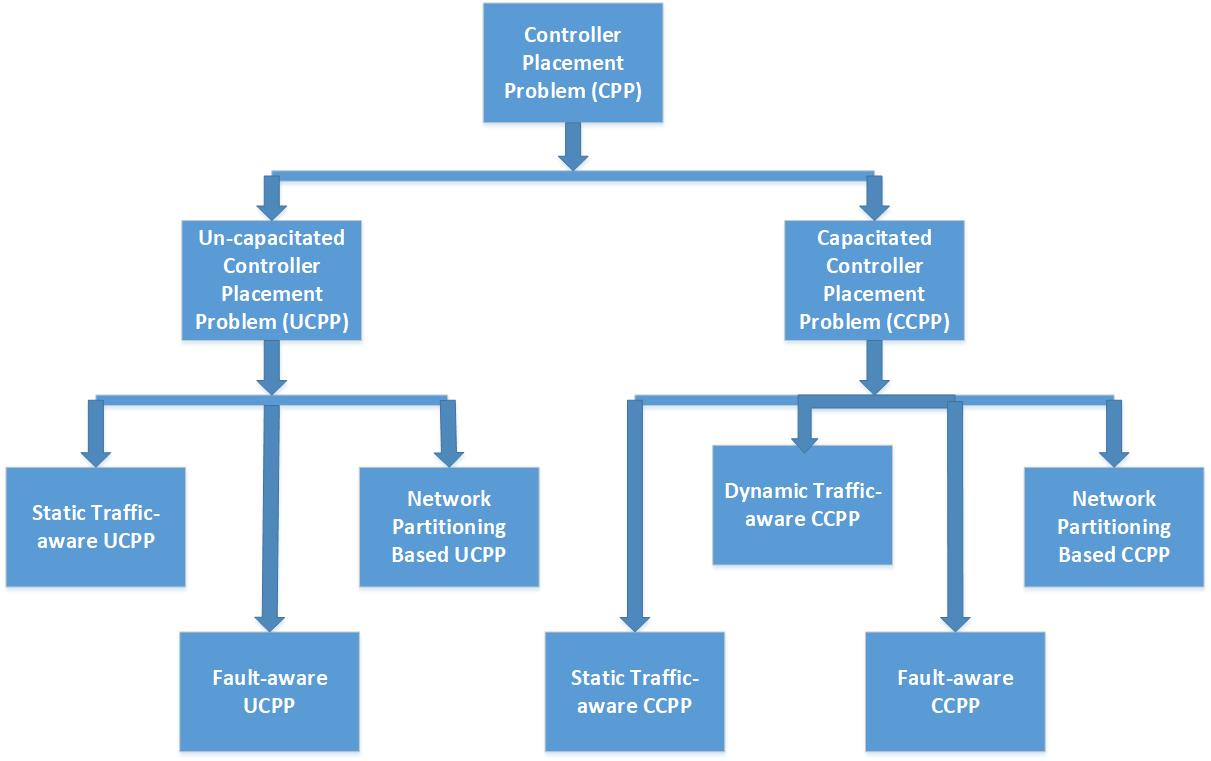
\includegraphics[width=\linewidth]{cppclassification.jpg}
	\caption{Classification of Controller Placement Problem (CPP)}
	\label{fig:cppclass}
\end{figure}

In the current decade many solutions have been proposed to solve this NP-Hard problem of controller placement \cite{cpp2012heller, cppsurvey2017, cppsurvey2018}. Heller et. al. \cite{cpp2012heller} propose a solution of CPP by selecting $k$ controllers to minimize the average and maximum latency of the network. Sallahi et. al. \cite{sallahi2015optimal} provide a mathematical model which simultaneously determines the controller numbers, locations and included switches while meeting some constraints. An example of this constraint could be the cost of installing a controller.

Yao et. al. \cite{yao2014capacitated} introduce capacitated controller placement. They consider the load or capacity of a controller and the load of switch, thus the capacity of a controller cannot be exceeded. Ozsoy et. al.\cite{ozsoy2006exact} propose an advanced version of the k-center algorithm using links between switches which is also a work on capacitated controller placement. In \cite{yao2015controller}, Yao et. al. uses flow algorithm to implement a dynamic solution which can work comfortably with changing data flows due to traffic or other reasons.

There are also notable research works on other parameters like reliability. Zhang et. al. \cite{zhang2011resilience} propose a solution which improves the resilience of a split architecture network. They improve the reliability of the network using Min-cut algorithm \cite{erlebach2006robustness} to find the fault tolerant and vulnerable parts of the network. There are also heuristic based approaches to solve the CPP problem. Lange et. al\cite{lange2015heuristic} propose a well-known algorithm named Pareto-based Optimal COntroller placement (POCO). POCO provides operators with pareto optimal placements with respect to different performance metrics. POCO performs an exhaustive evaluation of all possible placements by default, which is feasible for small networks. For large networks POCO uses heuristics which makes it faster but less accurate.


Liao et. al.\cite{dbcp2017} propose a faster algorithm named Density Based Controller Placement (DBCP). DBCP uses a threshold hop count to calculate the density of each switch in the network and then defines a distance for each switch which is the minimum distance to a higher density node and takes an average of these distances. If for some node or switch the minimum distance to higher density node is greater than the average distance then another controller is needed. In this way DBCP increments the value of $k$ from zero, which is the number of controllers, to a suitable value. Then keeping the switches which have a higher than average value of their minimum distance to higher density node as cluster heads, DBCP assigns the other switches to the clusters of their nearest higher density switch.

DBCP is a state-of-art-algorithm which outperforms the above mentioned algorithms that work on UCPP, but the distance metric used is hop count. If the goal is to create a programmable network that changes the flow path of data depending on network conditions (traffic, bandwidth etc.), then these parameters need to be considered and handled by the algorithm.

Our proposed algorithms are based on the well known algorithm SPICi (‘spicy’, Speed and Performance In Clustering) \cite{spici2010}, a fast clustering algorithm for biological networks, which divides a collection of proteins based on how closely they are related in terms of similarities\cite{protein2005palla}. The clusters that are formed contain closely connected proteins. SPICi clusters the network based on confidence values between two proteins and creates clusters that have maximum confidence values between them.

\section{Problem Formulation} \label{problemformulation}

Networks are distributed throughout the whole world. Each of them are of different types and topologies depending on the requirement. In SDN only the controllers take the routing decisions. Therefore, to demonstrate clustering, all the nodes are considered as switches (routers are replaced by switches).

We consider the network as a bi-directional graph $G=(S,L)$ consisting of nodes and edges. Here the set of nodes $S$ represent the switches and the set of edges $L$ represent the links between the switches. The edges can be either weighted or unweighted based on the requirements. Our objective is to cluster the graph $G$ into multiple sub-networks $S_{i:i=1,2,3...}$ such that each sub-network contains a set of switches $S_i=\{s_1,s_2,...\}$, where $s_1$, $s_2$ etc. are switches. There cannot be any common switch between two sub-networks and all of the switches of the network must fall into a sub-network, where each sub-network will have one and only one controller.

Let us assume that the network will be clustered into $k$ partitions. The sub-networks can be presented as,

\begin{equation} \label {eqn:clustering}
S_{net} \gets \{S_1=\{s_{1,1},s_{1,2},....s_{1,i}\},S_2,....,S_k\}
\end{equation}

where, $S_{net}$ is the total network and $S_1,S_2,...,S_k$ are $k$ disjoint sets of switches (sub-networks).

\section{Existing Algorithms} \label{existingalgo}
In this paper we focus on two existing clustering algorithms. One of them is Density Based Controller Placement (DBCP) and the other is SPICi. DBCP \cite{dbcp2017} is a recently proposed algorithm for clustering Software Defined Networks (SDN). SPICi\cite{spici2010} is a well known protein-clustering algorithm for biological networks. These algorithms are described in the following sections. 
\subsection{DBCP\cite{dbcp2017}}
This algorithm is named Density Based Controller Placement (DBCP) because it uses local density to calculate all other parameters of the algorithm and then clusters the algorithm using those parameters. The pseudo-code for clustering using DBCP is given in algorithm \ref{algo:dbcp}.
\subsubsection{Clustering} \label{dbcp:clustering}
DBCP uses the following equation to calculate the local density of each of the nodes in the network,
\begin{equation} \label{dbcp:density}
\rho_i=\sum_j\chi(d_{ij}-d_c)
\end{equation}
where, local density $\rho_i$ of a node $i$ is the count of all the nodes which are at most $d_c$ distance away from $i$. The threshold $d_c$ is a distance used to set a limit to the cluster diameter and consequently to find an approximate to the optimal value of $k$ where $k$ is the number of controllers.
Here $d_{ij}$ gives the minimum distance between nodes $i$ and $j$. The value of $\chi(x)$ is 1 only for $d_{ij}<d_c$ that is when $x<0$ and is 0 otherwise. Thus $\rho_i$ is the number of nodes that can be reached from node $i$ by traversing at most distance $d_c$.

The minimum distance of a node $i$ to a higher density node is represented by,
\begin{equation} \label{dbcp:mindistohi}
\delta_i=\begin{cases}
\max_{j:j\in S}(d_{ji}), & \text{if switch i has}\\ & \text{the highest $\rho_i$}\\
\min_{j:j\in S,\rho_j>\rho_i}(d_{ji}), & \text{otherwise}
\end{cases}
\end{equation}
where, $\delta_i$ is the minimum distance to a higher density node and $S$ is the set of all switches in the network. If $i$ is the node with highest density, $\delta_i$ holds the distance of the farthest node from $i$. Then an average of the minimum distance to higher density node $\delta_i$ is calculated for all nodes $i$ and denoted as $\delta$. The value of $k$, the number of controllers is initialized as $0$. If the value of $\delta_i$ of a node $i$ is greater than $\delta_i$, then $k$ is incremented. The switches with higher values of $\delta_i$ are selected as cluster heads of new clusters and the other switches are assigned to the nearest node with higher local density.


\begin{algorithm}
	\caption{DBCP}\label{algo:dbcp}
	\begin{algorithmic}[1]
		\Procedure{DBCP}{S,L} \\
		$k \gets 0$ \\
		\textbf{for $s$ in S:}
		\State $\rho_s=\sum_{j\in S}\chi(d_{sj}-d_c)$ \\
		\textbf{end for} \\
		\textbf{for $s$ in S:}
		\State $\delta_s=\min_{i:i\in S,p_i>p_s}(d_{is})$ \\
		\textbf{end for} \\
		$\delta \gets \frac{1}{|S|}\sum_{s\in S}\delta_s$ \\
		\textbf{for s in S:}
		\If {$\delta_s>\delta$}	
		\State $k = k + 1$
		\State $s \gets newcluster$
		\Else
		\State $s \gets cluster of nearest higher density$
		\EndIf \\
		\textbf{end for}
		\EndProcedure
	\end{algorithmic}
\end{algorithm}

\subsubsection{Controller Selection} \label{dbcp:consel}
DBCP uses the summation of three metrics to determine the controller for a cluster. The cluster head of a network is a node from where the cluster formation starts. A controller is the node which acts as the control plane. Each sub-network has it's own controller. These controllers send routing information to their respective data planes. The data plane of every sub-network consists of it's switches. These three metrics are $\pi^{avglatency}$, $\pi^{maxlatency}$ and $\pi^{inter\_controller}$.

For a sub-network $S_i$, is the average latency for a switch $v$ is calculated as follows:
\begin{equation}	\label{eqn:avglat}
\pi^{avglatency}(v)_{v:v\in S_i} = \frac{1}{|S_i|} \sum_{s\in S_i}d(v,s)
\end{equation}

This is the average of the distances of the node $v$ from all other nodes. It is the sum of all distances between $s$ and $v$ of cluster $S_i$ divided by the total number of switches in the cluster $|S_i|$.

For the worst case scenario the second metric is defined. This metric is denoted by $\pi^{maxlatency}$.
\begin{equation}	\label{eqn:maxlat}
\pi^{maxlatency}(v)_{v:v\in S_i} = \max_{s\in S_i}d(v,s)
\end{equation}

Here, $\pi^{maxlatency}(v)$ is the maximum of the distances of the node $v$ from all other nodes $s$ in the cluster $S_i$.

The inter controller latency must be reduced as much as possible when selecting controller. However, the controller to controller distance cannot be determined when the controllers are yet to be selected. Thus the third metric is used which calculates the distances from all other nodes that are not in the same cluster. It is an approximate calculation of the inter-controller distances and is denoted by $\pi^{inter\_controller}$.
\begin{equation}	\label{eqn:iclat}
\pi^{inter\_controller}(v)_{v:v\in S_i} = \frac{1}{|S-S_i|} \sum_{s\in (S-S_i)}d(v,s)
\end{equation}
$\pi^{inter\_controller}$ for a node $v$ is the sum of the distances between $v$ and all the nodes of other clusters. This sum is then divided by the total number of switches in the network that are in other clusters.

The final metric $\pi^{latency}(v)$ can be presented as follows by using three metrics in equations \ref{eqn:avglat}, \ref{eqn:maxlat} and \ref{eqn:iclat}.
\begin{equation}	\label{eqn:totlat}
\begin{split}
\pi^{latency}(v) = \pi^{avglatency}(v) + \pi^{maxlatency}(v) \\
 + \pi^{inter\_controller}(v)\\
 =\frac{1}{|S_i|} \sum_{s\in S_i}d(v,s) + \max_{s\in S_i}d(v,s) \\
 + \frac{1}{|S-S_i|} \sum_{s\in \{S-S_i\}}d(v,s)
\end{split}
\end{equation}
Here $\pi^{latency(v)}$ is the sum of all the three values of $\pi^{avglatency}(v)$, $\pi^{maxlatency}(v)$ and $\pi^{inter\_controller}(v)$ for a switch $v$. Then in each cluster, the switch with the minimum value of $\pi^{latency}$ is taken as the controller of that cluster.

\subsubsection{Complexity Analysis} \label{dbcp:compan}
There are two steps of DBCP. The first step, which is, finding the value of $k$, requires calculating the distances between all possible pair of nodes. Although in \cite{dbcp2017} this has not been mentioned, to the best of our knowledge this can be done with complexity $O(V(V+E))$ using Dijkstra's algorithm to calculate all possible pair distances between nodes, where $V$ is the number of nodes and $E$ is the number of edges. As this distance is only calculated once so it can be considered as pre-calculated and does not need to be included in complexity analysis.

Then calculating the value of $\rho_i$ or local density for all nodes $i$ has complexity $O(V^2)$ in the worst case when all other nodes are reachable by $d_c$ number of hops. Calculating the value of $\delta_i$ for all nodes has the same complexity. Increasing and assigning controllers has complexity of $O(V)$. Therefore if complexity is denoted by $\eta$ then the complexities can be written as follows:
\begin{equation}
\begin{split}
\eta_{dbcp} 
& = \eta_{\rho} + \eta_{\delta} + \eta_{k}\\
& =O(V^2) + O(V^2) + O(V)\\
& =O(V^2) \\
\end{split}
\end{equation}

Therefore after all the constants are canceled out, the complexity of DBCP is $O(V^2)$.

\subsection{Speed and Performance In Clustering (SPICi)\cite{spici2010}}
SPICi ('spicy', Speed and Performance In Clustering) clusters a connected undirected network $G=(V,E)$ with edges that have values of the continuous range $(0,1)$. It is named so because it is an extremely fast algorithm for clustering biological networks. The values of the edges are called confidence values, denoted by $w_{u,v}$ for adjacent nodes $u$ and $v$, and they represent similarities between two proteins \cite{protein2005palla}. The proteins are represented as nodes of the graph.

\subsubsection{Clustering}
SPICi clusters a network using three variables. They are the weighted degree of a node, the density for a set of nodes and the support for a node with respect to a set of nodes. The weighted degree of a node $u$ denoted by $d_w(u)_{u\in V}$ can be presented as:
\begin{equation} \label{eqn:spicidegree}
d_w(u)_{u\in V} = \sum_{v:v\in V,(u,v) \in E}w_{u,v}
\end{equation}

Here $d_w(u)_{u\in V}$ is the sum of all the confidence values of the edges that connect $u$ with any other adjacent node $v$ of the graph $G=(V,E)$. It is to be noted that only those nodes are considered which are still unclustered. The density of a set of nodes denoted by density(S), can be presented as:

\begin{equation} \label{eqn:spicidensity}
density(S) = \frac{\sum_{(u,v)\in E}w_{u,v}}{|S|*(|S|-1)/2} 
\end{equation}

In other words, $density(S)$ is the sum of the confidence values of the edges that connect every node $u$ with every other node $v$ of the set of nodes $S$, divided by the number of total possible nodes that is $|S|*(|S|-1)/2$ where $|S|$ is the number of nodes present in the set of nodes $S$. The support of a node $u$ with respect to a set of nodes $S$ can be presented as:

\begin{equation} \label{support}
support(u,S) = \sum_{v\in S} w_{u,v}
\end{equation}
For a network, $support(u,S)$ is the sum of the confidence values of the edges that connect a node $u$ with the nodes that are adjacent to it and are present in the set of nodes $S$.

\begin{algorithm}
	\caption{: SPICi}\label{spicicode}
	\begin{algorithmic}[1]
		\Procedure{Search}{} \\
		Initialize \textbf{DegreeQ} to be $V$ \\
		While \textbf{DegreeQ} is not empty
		\State Extract $u$ from \textbf{DegreeQ} with largest weighted degree
		\If {$u$ has adjacent vertices in \textbf{DegreeQ}}
		\State 1. Find from $u$’s adjacent vertices the second seed protein v (see text)
		\State 2. $S=Expand(u,v)$
		\Else 
		\State $S=\{u\}$
		\EndIf
		\State $V=V-S$
		\State Delete all vertices in S from \textbf{DegreeQ}
		\State For each vertex t in \textbf{DegreeQ} that is adjacent to a vertex in $S$, decrement its weighted degree by $support(t,S)$
		\EndProcedure
	\end{algorithmic}
\end{algorithm}

Using these parameters, SPICi clusters a network as given in the algorithm \ref{spicicode}.
The first seed is the node with the maximum weighted degree. 
After the selection of the first seed, the adjacent nodes are divided into five bins depending on the confidence value of the connecting edge. The bins are of ranges $(0:0.2:0.4:0.6:0.8:1)$, that is, they are at regular intervals of $0.2$ in the already given range $(0,1)$. Then starting from the maximum bin $(0.8:1)$, the node with the maximum weighted degree, $d_w$ is taken as the second seed.

SPICi uses two thresholds. These thresholds are: $T_s$ which determines whether a node is to be included in the cluster based on the cluster size and the connectivity of the node to the cluster and: $T_d$ which includes a node to the cluster, based on the density increased when the node is added. The algorithm gives better results when these thresholds have a value of 0.5\cite{spici2010}.

\begin{algorithm}
	\caption{: SPICi EXPAND function}\label{spiciexpand}
	\begin{algorithmic}[1]
		\Procedure{Expand}{u,v}\\
		Initialize the cluster $S=\{u,v\}$
		Initialize \textbf{CandidateQ} to contain vertices neighboring $u$ or $v$
		While \textbf{CandidateQ} is not empty
		\State Extract from \textbf{CandidateQ} with highest $support(t,S)$
		\If {$support(t,S)\geq T_s*|S|*density(S)$ and $density(S+{t})>T_d$}
		\State $S=S+{t}$
		\State Increase the support for vertices connected to t in
		\textbf{CandidateQ}
		\State For all unclustered vertices adjacent to t, insert them
		into \textbf{CandidateQ} if not already present
		\Else
		\State break from loop
		\EndIf \\
		\textbf{return} S
		\EndProcedure
	\end{algorithmic}
\end{algorithm}

As SPICi is a clustering algorithm that works on biological networks it does not select any controller for any cluster. It only selects first seed and second seed and includes the nodes in each cluster. Therefore there is no Controller Selection step for SPICi.

\subsubsection{Complexity Analysis}
SPICi can be divided into three phases or functions. The first function selects the first seed from a sorted queue which has time complexity of $O(Vlog_2(V+E))$ in the worst case when all nodes are connected to all other nodes. The second function or second seed selection process requires $O(V)$ time complexity as all the weighted degrees have already been calculated in the first seed selection phase. The expand function (Algorithm \ref{spiciexpand}) calculates the support value for each node in the CandidateQ which is a sorted queue or priority queue. Therefore this phase requires a complexity of $O(Vlog_2(V+E))$.

Let the complexity of the algorithm be denoted by $\eta^{SPICi}$. Then the complexities can be calculated in the following manner.
\begin{equation}
\begin{split}
\eta^{SPICi} &= \eta^{f\_seed} + \eta^{s\_seed} + \eta^{expand}\\
&= Vlog_2(V+E) + O(V) + Vlog_2(V+E)\\
&=Vlog_2(V+E)
\end{split}
\end{equation}

Thus complexity of SPICi is $Vlog_2(V+E)$ which shows how fast this algorithm is.

\section{Proposed Algorithms} \label {proposedalgo}
We propose four algorithms to address the Controller Placement Problem for both unweighted and weighted network. One of our proposed algorithms work on unweighted graphs and we name it Random Clustering with Local Search (RCLS). Rest of the three is for weighted graph and we name them Greedy-SPICi (G-SPICi), Inverse SPICi (I-SPICi) and Modified-SPICi (M-SPICi).

\subsection{Random Clustering with Local Search (RCLS)}
This algorithm is only for networks that have hop count as metric, that is all the edge weights of the graph are set to one. Therefore it has the same working conditions as DBCP.
\subsubsection{Clustering} \label{rcls:clustering}
We chose $k$ random cluster heads where the value of $k$ is fixed. We assign every other node to the cluster whose cluster head has the shortest distance from that node. Then we optimize it using local search. We perform local search by including one randomly selected node in a randomly selected cluster in each iteration until latency of the network cannot be decreased anymore. The latency of the network in this case is calculated using the metric defined for evaluating DBCP (equation \ref{eqn:metric}).

\begin{algorithm}
	\caption{: RCLS}\label{rcls}
	\begin{algorithmic}[1]
		\Procedure{RCLS}{k, iteration} \\
		Randomly select $k$ cluster heads from the graph \\
		Include all switches to nearest cluster heads \\
		latency $\gets$ calculate latency of current network \\
		\textbf{for i = 1 to iteration}
		\State Local\_Search(latency) \\
		\EndProcedure
		
		\Procedure {Local\_Search}{latency} \\
		\textbf{for i = 1 to n*k}
		\State $a$ = randomly choosen node from the garph.
		\State $b$ = randomly chosen cluster from the cluster set.
		\If {already checked for pair($a$,$b$)}
		\State continue.
		\EndIf
		\State Swap the cluster of $a$ to $b$.
		\State set new controller heads
		\If {$new m_{latency} < latency$}
		\State $latency \gets new m_{latency}$
		\State \textbf{break}
		\Else 
		\State set the cluster of $a$ to it's previous cluster
		\EndIf
		\EndProcedure
	\end{algorithmic}
\end{algorithm}

\subsubsection{Controller Selection}
In each iteration it selects $k$ controllers and after evaluating it again selects $k$ controllers for the changed graph when the random node is put in a random cluster. The controller selection method is same as DBCP (section \ref{dbcp:consel}).

All the distances used in this algorithm are hop counts, which is same as that of DBCP.
Therefore this algorithm can be only applied to un-weighted graphs.

\subsubsection{Complexity Analysis}
RCLS randomly selects $k$ nodes as cluster heads, provided that $k$ is given. This step has complexity of $k$. Each node needs to be included in a cluster which requires a complexity of $k\times n$ if $n$ is the total number of nodes. For local search the algorithm randomly selects cluster and randomly selects a node and puts the node in the cluster to check $m_{latency}$. The calculation of $m_{latency}$ has complexity of $n^3$. In the worst case when a better solution does not exist, the algorithm calculates $m_{latency}$ for all possible pairs. This has a complexity of $k\times n$.
\begin{equation}
\begin{split}
\eta^{RCLS} &= \eta^{cluster} + \eta^{local\_search} \\
&= O(k\times n) + O(k\times n \times n^3) \\
&= O(k\times n^4) \\
\end{split}
\end{equation}

\subsection{Greedy-SPICi}
Greedy-SPICi (G-SPICi) is a variation of SPICi. G-SPICi does not divide the nodes connected to the first seed into bins as done in SPICi. After selecting the first seed, G-SPICi starts clustering with the nodes adjacent to the first seed. The nodes are selected greedily based on their support value (equation \ref{support}) with respect to the whole network, hence we named the algorithm Greedy-SPICi (Algorithm \ref{gspicicode}).
\subsubsection{Clustering}
G-SPICi starts with a node having maximum weighted degree and then forms a cluster including it's neighboring nodes using an expand function (algorithm \ref{gspiciexpand}).
In the \emph{EXPAND} function the nodes adjacent to the first seed are sorted based on a support value with respect to the present cluster being formed. For example when the \emph{EXPAND} function is called, the present cluster consists of only first seed $u$ (line 8 of algorithm \ref{gspicicode}).
\begin{algorithm}
	\caption{: G-SPICi}\label{gspicicode}
	\begin{algorithmic}[1]
		\Procedure{Search}{V,E} \\
		\textbf{Initialize} $DegreeQ = V$ \\
		\textbf{While} $DegreeQ \neq empty$
		\State Extract u from DegreeQ with largest $d_w(u)$
		\If {there is $v_{v:v,u\in E}\in DegreeQ$}
		\State $S \gets Expand(v)$
		\Else 
		\State $S \gets \{u\}$
		\EndIf
		\State $V \gets V - S $
		\State $Degree Q \gets Degree Q - S$
		\State $d_w(t)_{t:t\in DegreeQ,(t,s)_{s\in S}\in E} = d_w(t) - support(t,S)$
		\EndProcedure
	\end{algorithmic}
\end{algorithm}


G-SPICi initializes a priority queue called $DegreeQ$ that holds the degree of each node using equation \ref{eqn:spicidegree}. From $DegreeQ$ the node with the highest weighted degree is extracted and the cluster is expanded using expand function. The nodes present in the formed cluster is then removed from $DegreeQ$ and the support value of rest of the nodes are updated accordingly. This process continues until there is no more nodes left in $DegreeQ$.

The \emph{EXPAND} function starts with forming the cluster $S$ from first seed $u$. The nodes adjacent to the present cluster are the candidates of being included in the cluster they form the candidate list. A priority queue $CandidateQ$ is formed from the support values of the members of the candidate list. Each member of the candidate list is then included in the cluster based on a conditional statement (line 6 of algortihm \ref{gspiciexpand}). If the node is included in the cluster then the node is removed from $CandidateQ$ and it's adjacent nodes are inserted into $CandidateQ$ except the ones that are already there, and the support values of the nodes in $CandidateQ$ are updated accordingly.

\begin{algorithm}
	\caption{: G-SPICi EXPAND function}\label{gspiciexpand}
	\begin{algorithmic}[1]
		\Procedure{Expand}{V,E,u}\\
		\textbf{Initialize} the cluster $S \gets \{u\}$ \\
		\textbf{Initialize} $CandidateQ = S_{S:s\in S,(s,u)\in E}$\\
		\textbf{While} $CandidateQ \neq empty$
		\State Extract $t$ from Candidate with highest $support(t,S)$
		\If {$support(t,S)\geq T_s*|S|*density(S)$ and
			$density(S + t)> T_d$}
		\State $S\gets S+\{t\}$
		\State $CanditateQ \gets CandidateQ + \{s_{s:(s,t)\in E}\}$
		\State $CandidateQ \gets CandidateQ - \{s_{s:s\not\in CandidateQ}\}$
		\Else
		\State break from loop
		\EndIf \\
		\Return S
		\EndProcedure
	\end{algorithmic}
\end{algorithm}
\subsubsection{Controller Selection}
The controller selection process of G-SPICi is same as that of DBCP except that it uses edge weights (positive integers) to calculate the three metrics $\pi^{avglatency}$, $\pi^{maxlatency}$ and $\pi^{inter\_controller}$, mentioned in section \ref{dbcp:consel}, instead of hop counts. As a result the controllers are selected such that the controller-to-switch and controller-to-controller latencies are minimized where the latencies are integer values.

\subsubsection{Complexity Analysis}
G-SPICi has the same complexities as SPICi, only the second seed selection is omitted and local search is added. If $n$ is the total number of nodes and $m$ is the total number of edges. Then the complexity of G-SPICi can be denoted by $\eta^{G-SPICi}$ where,
\begin{equation}
\begin{split}
\eta^{G-SPICi} &= \eta^{f\_seed} + \eta^{expand} + \eta^{local\_search}\\
&= 2nlog_2(n+m)+O(k\times n^4)\\
&= O(k\times n^4)\\
\end{split}
\end{equation}

\subsection{Inverse-SPICi}

Inverse-SPICi (I-SPICi) is a variation of G-SPICi. I-SPICi converts the edge weights of the network such that the highest edge weight becomes the lowest edge weight and vice versa. SPICi forms clusters such that the connection among the nodes of the clusters are maximized where the edge weights are the similarity values. However, our goal is to minimize latency where the edge weights represent the latencies. This is why we invert the edge weights and name this algorithm Inverse-SPICi.
\subsubsection{Clustering}
I-SPICi inverts the edge weights. If the weight of an edge is $w$ and the maximum edge weight of the whole network is $w_{max}$, then the weight is inverted as follows:
\[
w_{inverted} = w_{max} - w + 1
\]

Here $w_{inverted}$ is the final edge weight. We subtract edge weight $w$ from maximum edge weight $w_{max}$, and add $1$ so that the maximum edge weight is not inverted to $0$.
\subsubsection{Controller Selection}
The controller selection process of G-SPICi and I-SPICi are identical. For this step the original edge weights are used and not the inverted weights.
\subsubsection{Complexity Analysis}
I-SPICi has the same complexities as G-SPICi, only the costs are inverted which requires a complexity of $m$, where $n$ is the total number of nodes and $m$ is the total number of edges. The complexity of I-SPICi is denoted by $\eta^{I-SPICi}$ where,
\begin{equation}
\begin{split}
\eta^{I-SPICi} &= \eta^{invert} + \eta^{G-SPICi}\\
&= O(m)+O(k\times n^4)\\
&= O(k\times n^4 + m)\\
\end{split}
\end{equation}
\subsection{Modified-SPICi}
M-SPICi or Modified SPICi is similar to the original SPICi. It includes some more steps, like pre-processing and post-processing and thus is named Modified-SPICi.

\subsubsection{Clustering}
Initially before starting the algorithm the degree of incidence (both outgoing and ingoing) of all the nodes are calculated. Then all the nodes are divided into five partitions based on their degree values in from highest to lowest. Thus the nodes in the first partition out of the five are of highest degree and have the highest probability of becoming first seed proteins. We named this partition seed partition.

All the edge costs $w$ are changed to $1/w$. This causes the edge values which are positive integers, are inverted and mapped to the range of SPICi, that is the continuous range $(0,1)$, at the same time using this single operation.

\begin{algorithm}
	\caption{: M-SPICi}\label{mpicicode}
	\begin{algorithmic}[1]
		\Procedure{Search}{V,E} \\
		\textbf{Initialize} $DegreeQ = V$ \\
		\textbf{While} $DegreeQ \neq empty$
		\State Extract u from DegreeQ with largest $d_w(u)$
		\If {there is $v_{v:v,u\in E}\in DegreeQ$}
		\State $v \gets secondseed(DegreeQ,E,u)$
		\If {$v\neq null$} $S \gets Expand(u,v)$
		\EndIf
		\Else 
		\State $S \gets \{u\}$
		\EndIf
		\State $V \gets V - S $
		\State $Degree Q \gets Degree Q - S$
		\State $d_w(t)_{t:t\in DegreeQ,(t,s)_{s\in S}\in E} = d_w(t) - support(t,S)$
		\EndProcedure
	\end{algorithmic}
\end{algorithm}

After the selection of the second seed M-SPICi starts expanding just like SPICi. When a node is found which does not meet the condition (line 6 of algorithm \ref{mspiciexpand}) for including in the cluster, the rest of the nodes in $CandidateQ$ are not discarded. These nodes are included in the cluster based on another condition check. For each node remaining in the $CandidateQ$ this check is performed. If the degree of the node is in the seed partition then this node is discarded as it can form a new cluster. The rest of the nodes are included in the cluster.

When all the nodes are clustered in this way, some isolated nodes remain. These are included in the adjacent clusters of the nearest first seeds or cluster heads.

\begin{algorithm}
	\caption{: M-SPICi second seed selection}\label{mpicisecond}
	\begin{algorithmic}[1]
		\Procedure{SecondSeed}{V,E,u} \\
		$bin[i]_{i:i=(1,5)} \gets s_{s:s\in V,(s,u)\in E}$ \\
		\textbf{for i = 1 to 5}
		\If {$bin[i] \neq empty$}
		\State \Return $v$ \textbf{if} $d_w(v)=\max_{s:s\in bin[i]}{d_w(s)}$
		\EndIf\\
		\Return $null$
		\EndProcedure
	\end{algorithmic}
\end{algorithm}
\begin{algorithm}
	\caption{: M-SPICi EXPAND function}\label{mspiciexpand}
	\begin{algorithmic}[1]
		\Procedure{Expand}{V,E,u,v}\\
		\textbf{Initialize} the cluster $S \gets \{u,v\}$ \\
		\textbf{Initialize} $CandidateQ = S_{S:s\in S,(s,u),(s,v)\in E}$\\
		\textbf{While} $CandidateQ \neq empty$
		\State Extract $t$ from Candidate with highest $support(t,S)$
		\If {$support(t,S)\geq T_s*|S|*density(S)$ and
			$density(S + t)> T_d$}
		\State $S\gets S+\{t\}$
		\State $CanditateQ \gets CandidateQ + \{s_{s:(s,t)\in E}\}$
		\State $CandidateQ \gets CandidateQ - \{s_{s:s\not\in CandidateQ}\}$
		\Else
		\State break from loop
		\EndIf \\
		\Return S
		\EndProcedure
	\end{algorithmic}
\end{algorithm}

\subsubsection{Controller Selection}
Controller Selection of M-SPICi is identical to G-SPICi. The original edge weights are used here.

\subsubsection{Complexity Analysis}
Assume the number of clusters is $k$, and the number of nodes and edges are respectively $n$ and $m$. M-SPICi has an edge weight inversion step of complexity $O(m)$. There is another pre-processing which calculates the degree of all nodes and sorts them. This step has complexity $O(m+nlog_2(n))$. The discarded nodes of $CandidateQ$ are processed but even including that the complexity is same as SPICi. The post-processing step for assigning isolated nodes is $O(n\times k)$. And the local search has complexity $O(k\times n^4)$. Therefore the total complexity is:
\begin{equation}
\begin{split}
\eta^{M-SPICi} &= \eta^{SPICi} + \eta^{processings} + \eta^{local\_search}\\
&= nlog_2(n+m)+O(m)+O(n\times k)\\&+O(m+nlog_2(n))+O(k\times n^4)\\
&= O(m+nlog_2(n+m)+k\times n^4)
\end{split}
\end{equation}

\subsection{Example Network}

In figure \ref{fig:example} the graph presented is one of the networks that we experimented on. It is an actual network that expands throughout the different states of USA and Canada, and are used for research purposes. We assigned random weights to the links between the switches. We applied our proposed algorithms on this network. For example, M-SPICi clusters the network into 9 sub-networks. The controllers of the sub-networks are 2,28,21,6,27,8,12,16 and 24 according to our simulation results. They give values 361.876, 724.166, 448, 495.133, 584.29, 664.172, 443.35, 322.625 and 430.25 respectively for their controller selection metric (equation \ref{eqn:totlat}). For each cluster, these are the switches which when selected as per the selection metric, give the best results. The latency of the network, $m_{latency}$ after clustering is 178.616. Therefore the cost-latency product is 1607.544.
\begin{figure}
	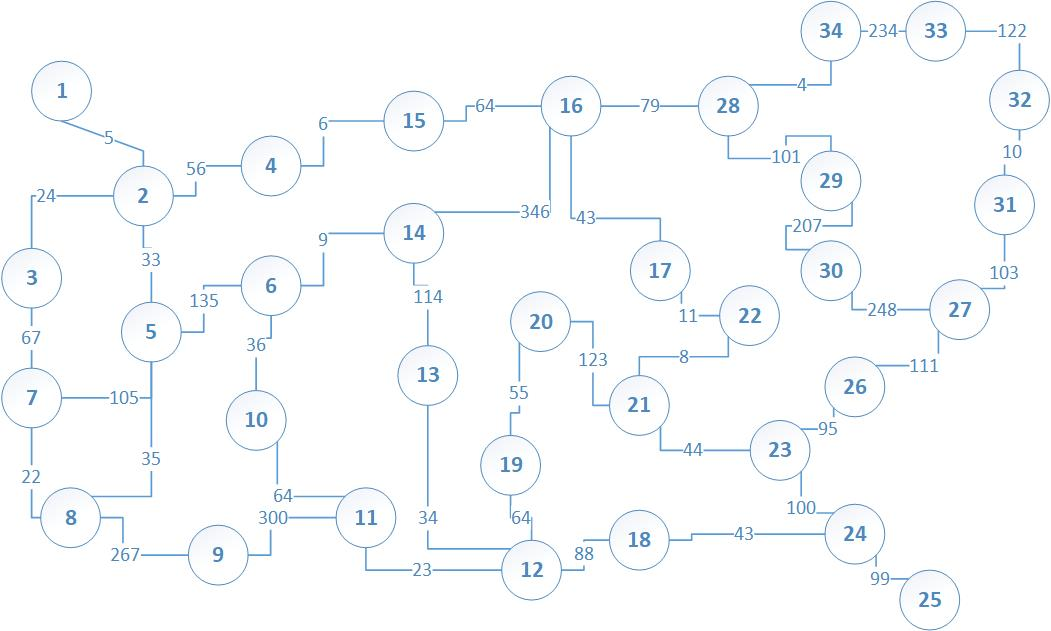
\includegraphics[width=\linewidth]{example.jpg}
	\caption{The Internet2 OS3E Network with 34 nodes and 42 edges expanding over Canada and USA used mainly for research purposes}
	\label{fig:example}
\end{figure}

\section{Performance Evaluation} \label {performance}
\subsection{Simulation Environment}
We performed all our experiments using the language C++. We use seven randomly generated networks with number of switches starting from 40 to 100, at regular intervals of 10. The edge to node ratio were kept from 1.1 to 1.4 to keep the networks considerably sparse as are found in current worldwide networks. The seven scenarios are shown in the table \ref{table:networks}. The graphs do not contain any self-loops or multi-edge. The graph may have cycles.
\begin{table}
	\begin{center}
		\textbf{\caption{Randomized Networks used as Input} \label{table:networks}}
		\begin{tabular}{|l|c|c|l|}
			\hline
			Scenario & Nodes & Edges & Edge/Node \\
			\hline
			1 & 40 & 52 & 1.3\\
			2 & 50 & 68 & 1.36\\
			3 & 60 & 77 & 1.2833\\
			4 & 70 & 87 & 1.2429\\
			5 & 80 & 108 & 1.35\\
			6 & 90 & 120 & 1.3333\\
			7 & 100 & 131 & 1.31\\
			\hline
		\end{tabular}
	\end{center}
\end{table}
We have simulated a number of scenarios but for convenience we have showed seven scenarios here in table \ref{table:networks}.
\subsection{Performance Metric}
In Software Defined Network, each time a new packet arrives, the switch asks the controller for decision. The controller decides the path of the packet and sends the routing information to all the switches in the path. If the switch is of another cluster then the information is sent to all the controller of that cluster. In \cite{dbcp2017}, J. Liao et. al. use this process to define a latency for a network denoted by $m_{latency}$.

\begin{equation} \label{eqn:metric}
\begin{split}
m_{latency} =& \frac{1}{|S|(|S|-1)}\sum_{s_i,s_j\in S, i\neq j}\{d(s_i,v_i)+\\
&\max_{s_m \in Path_{i,j}}(d(v_i,v_m)+d(v_m,s_m))\}
\end{split}
\end{equation}

Here, $|S|$ is the number of switches in the network, $s_i$ and $s_j$ are any two switches in that network. $v_i$ and $v_m$ are the controllers of the switches $s_i$ and $s_j$ respectively. The term $Path_{i,j}$ means the series of connected nodes that are in between nodes $s_i$ and $s_j$.

Thus the latency for a pair of switches is the sum of the distance from the initializing switch $s_i$ and the corresponding controller $v_i$, $d(v_i,v_m)$, and the maximum of the addition of the distances between the corresponding controller $v_i$, and the controllers of the switches of the path $v_m$, and the distances between the switches of the path $s_m$ and their controllers $v_m$, $max(d(v_i,v_m)+d(v_m,s_m))$.
\subsection{Result Comparison}


\begin{figure}
	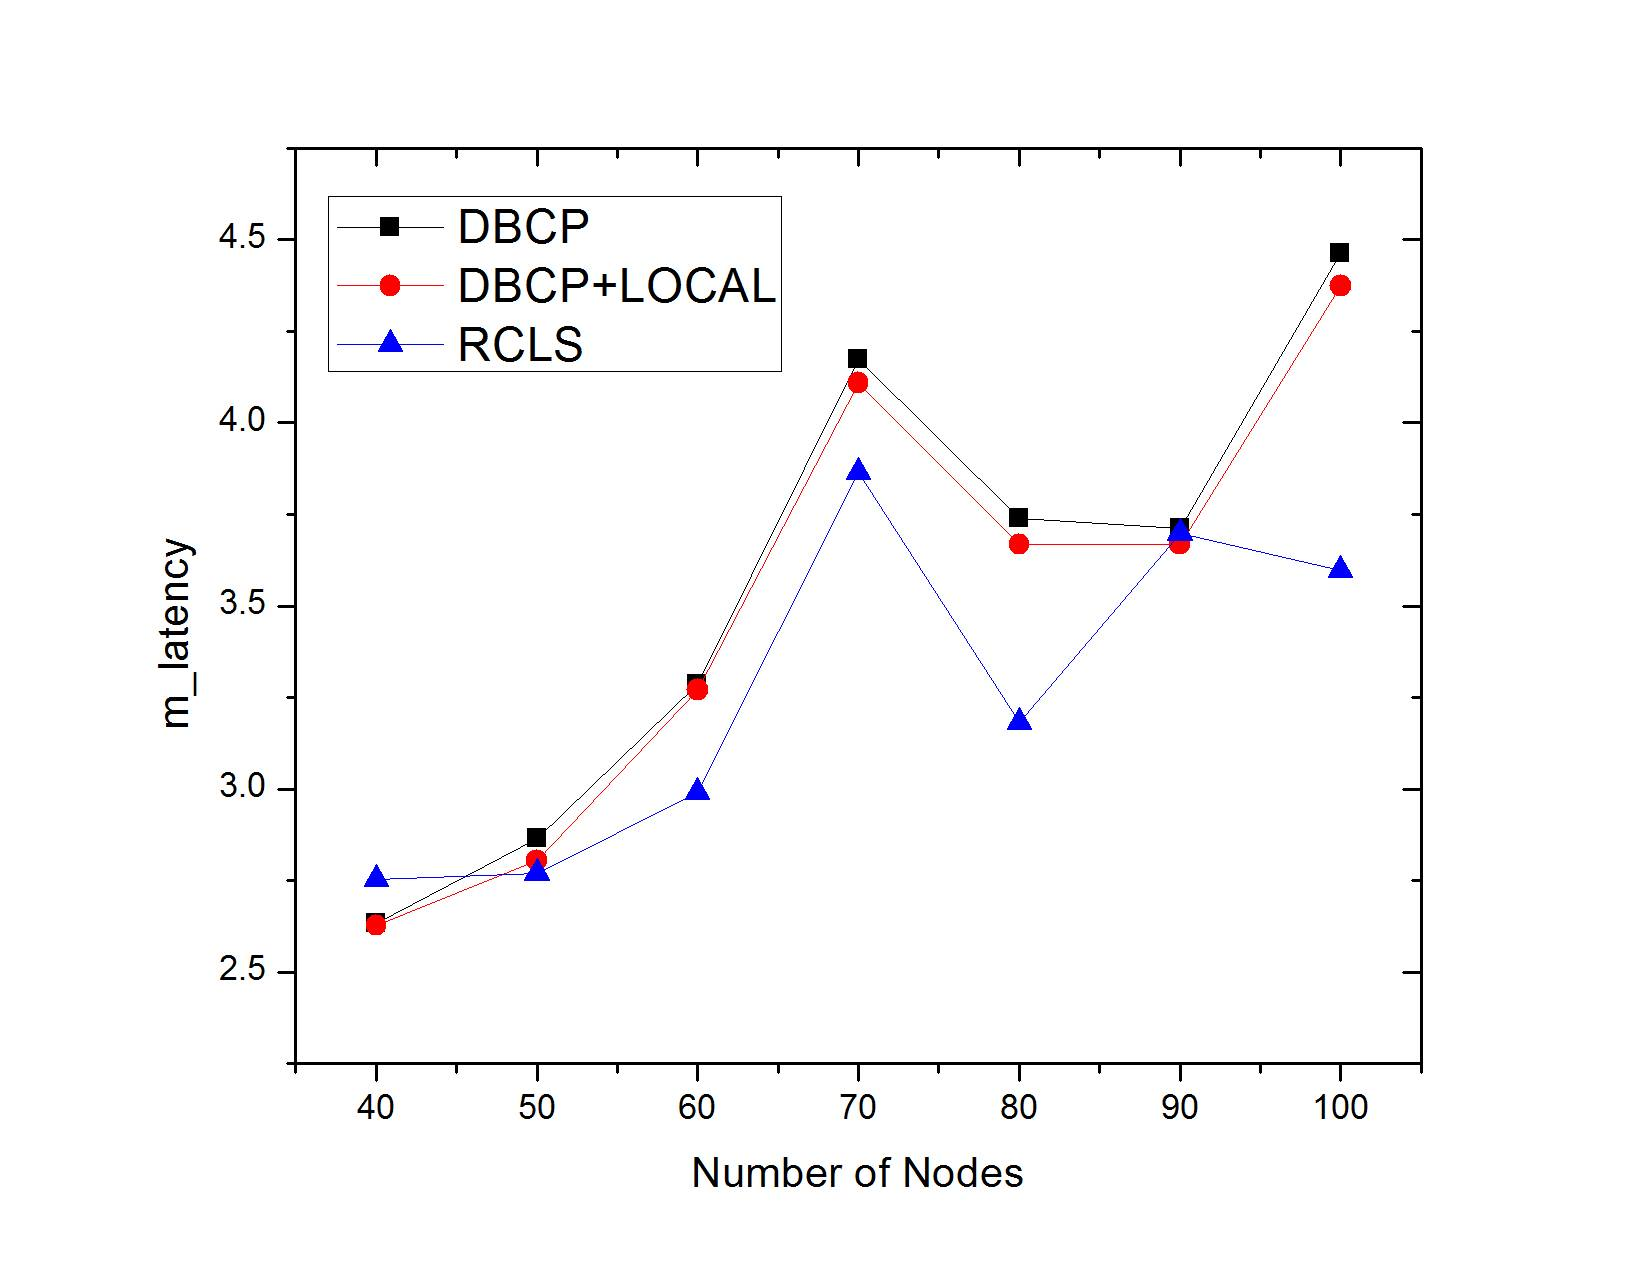
\includegraphics[width=\linewidth]{ugraph.jpg}
	\caption{Comparison of DBCP, DBCP with local search and RCLS on un-weighted networks using $m^{latency}$ as performance metric. The distances were calculated using hop count. As a result the unit of the y-axis, that is, of $m^{latency}$ is hop count. All these algorithms create the same number of clusters.}
	\label{fig:ugraph}
\end{figure}


We propose algorithms for both weighted and un-weighted networks. Initially we present a comparison between well-known algorithm DBCP, our proposed algorithm RCLS and a local search applied version of DBCP in un-weighted networks. Then for weighted networks where the edge values have been randomly assigned, we will evaluate and compare the algorithms G-SPICi, I-SPICi and M-SPICi with well-known algorithm DBCP. As DBCP works well using hop count, we used another weighted version of DBCP called W-DBCP as another algorithm for comparison.

Thus the results are divided into un-weighted and weighted comparison. The networks are same for both cases except for un-weighted graphs, the edge weights are set to one. The networks used for experimenting are given in table \ref{table:networks}.


\subsubsection{Result Comparison for Un-weighted Graph}
We propose RCLS for un-weighted graph. In figure \ref{fig:ugraph} we compare our proposed algorithm RCLS with existing algorithm DBCP. RCLS outperforms DBCP in terms of $m_{latency}$ for the same value of $k$. Furthermore, we applied local search on DBCP. In the simulation graph \ref{fig:ugraph} we represented it as DBCP+LOCAL. RCLS also outperforms DBCP+LOCAL in terms of $m_{latency}$.
		
\begin{figure}
	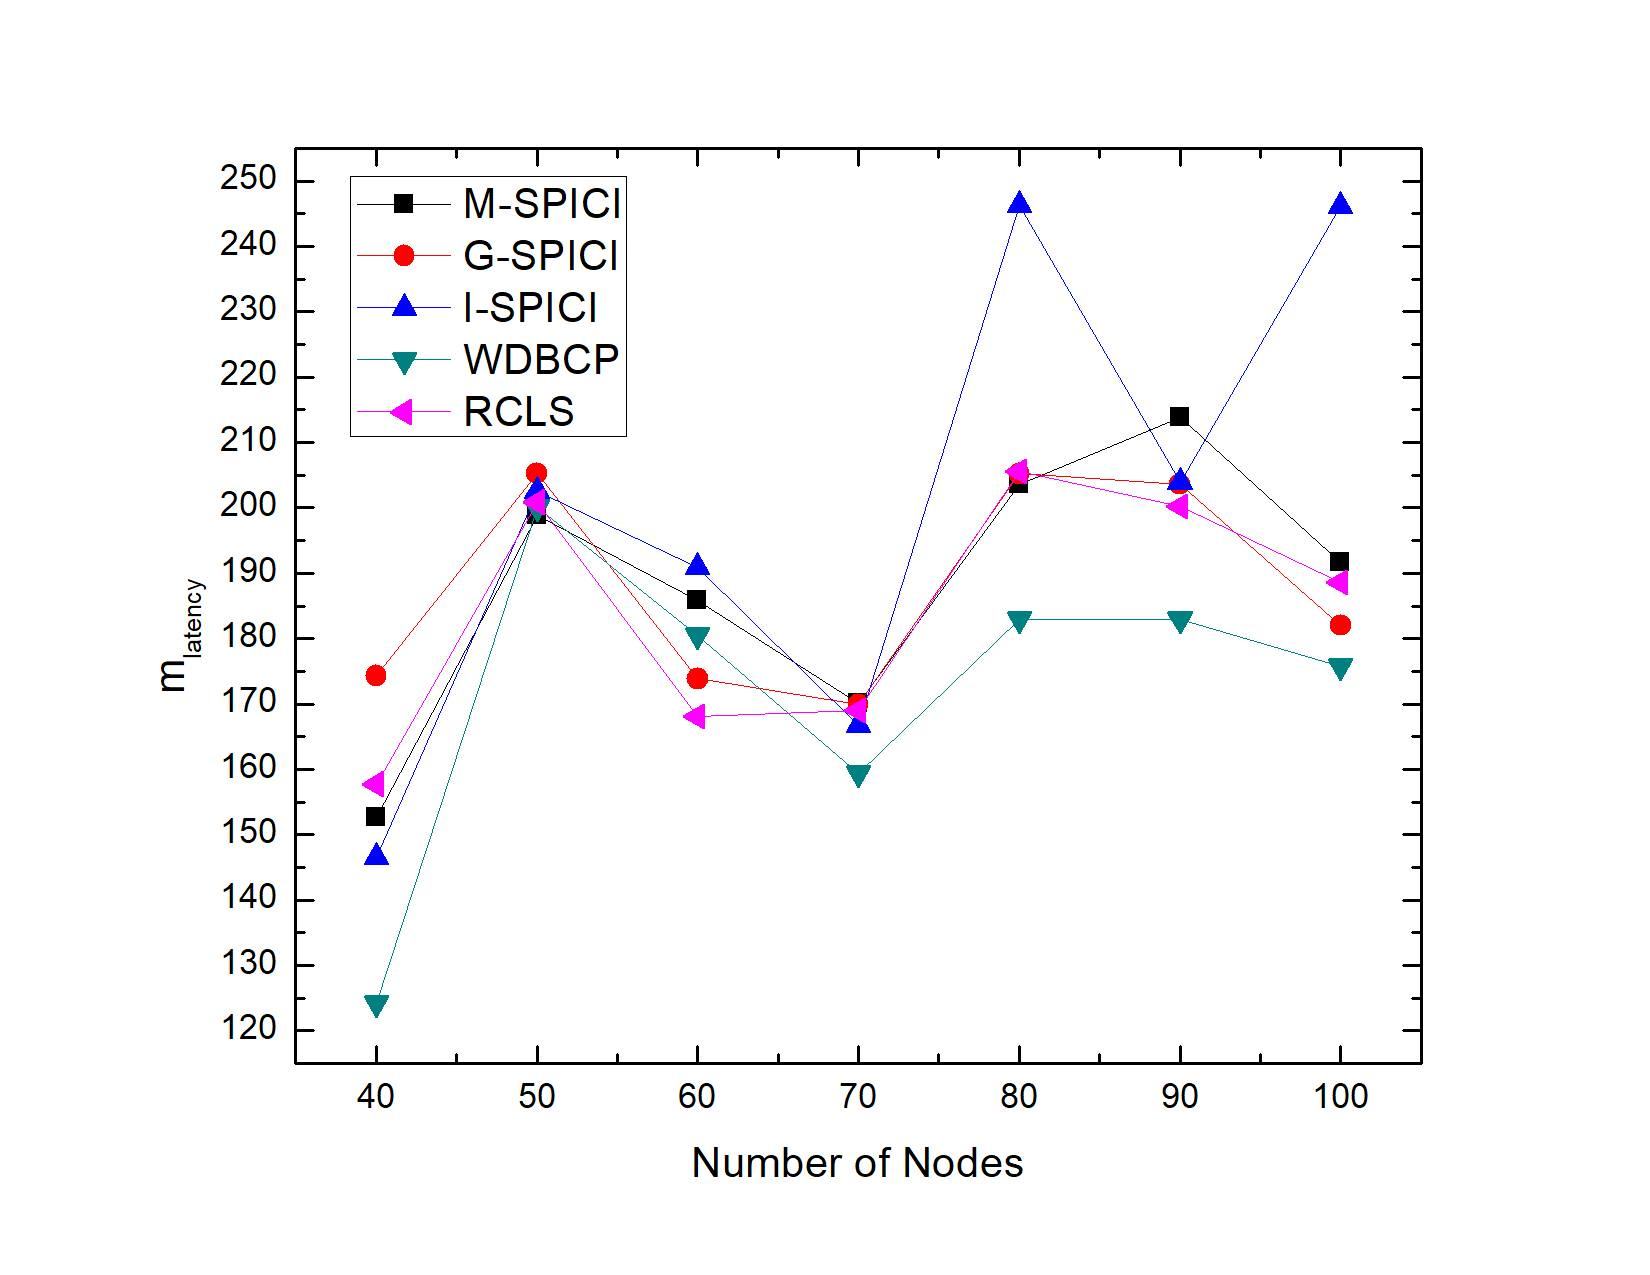
\includegraphics[width=\linewidth]{wgraph.jpg}
	\caption{Comparison of WDBCP, G-SPICi, I-SPICi and M-SPICi on weighted graphs using $m^{latency}$ as performance metric, where WDBCP is the implementation of DBCP using edge weights to calculate the distances instead of hop metric.}
	\label{fig:wgraph}
\end{figure}


We observe from figure \ref{fig:ugraph} that only for the $1^{st}$ scenario (table \ref{table:networks})where number of nodes is 40, RCLS gives greater latency than DBCP and DBCP+LOCAL. RCLS, DBCP and DBCP+LOCAL give almost equal latencies for scenario 6 only where number of nodes is 90. In all other scenarios RCLS outperforms both DBCP and DBCP+LOCAL.


\subsubsection{Result Comparison for Weighted Graph}
We propose three algorithms for weighted graphs which are G-SPICi, I-SPICi and M-SPICi. RCLS can also be implemented on weighted graph. We compare our proposed algorithms with weighted-DBCP. In the figure \ref{fig:wgraph} we represent weighted-DBCP as WDBCP, which considers edge weights instead of hop count.


\begin{figure}
	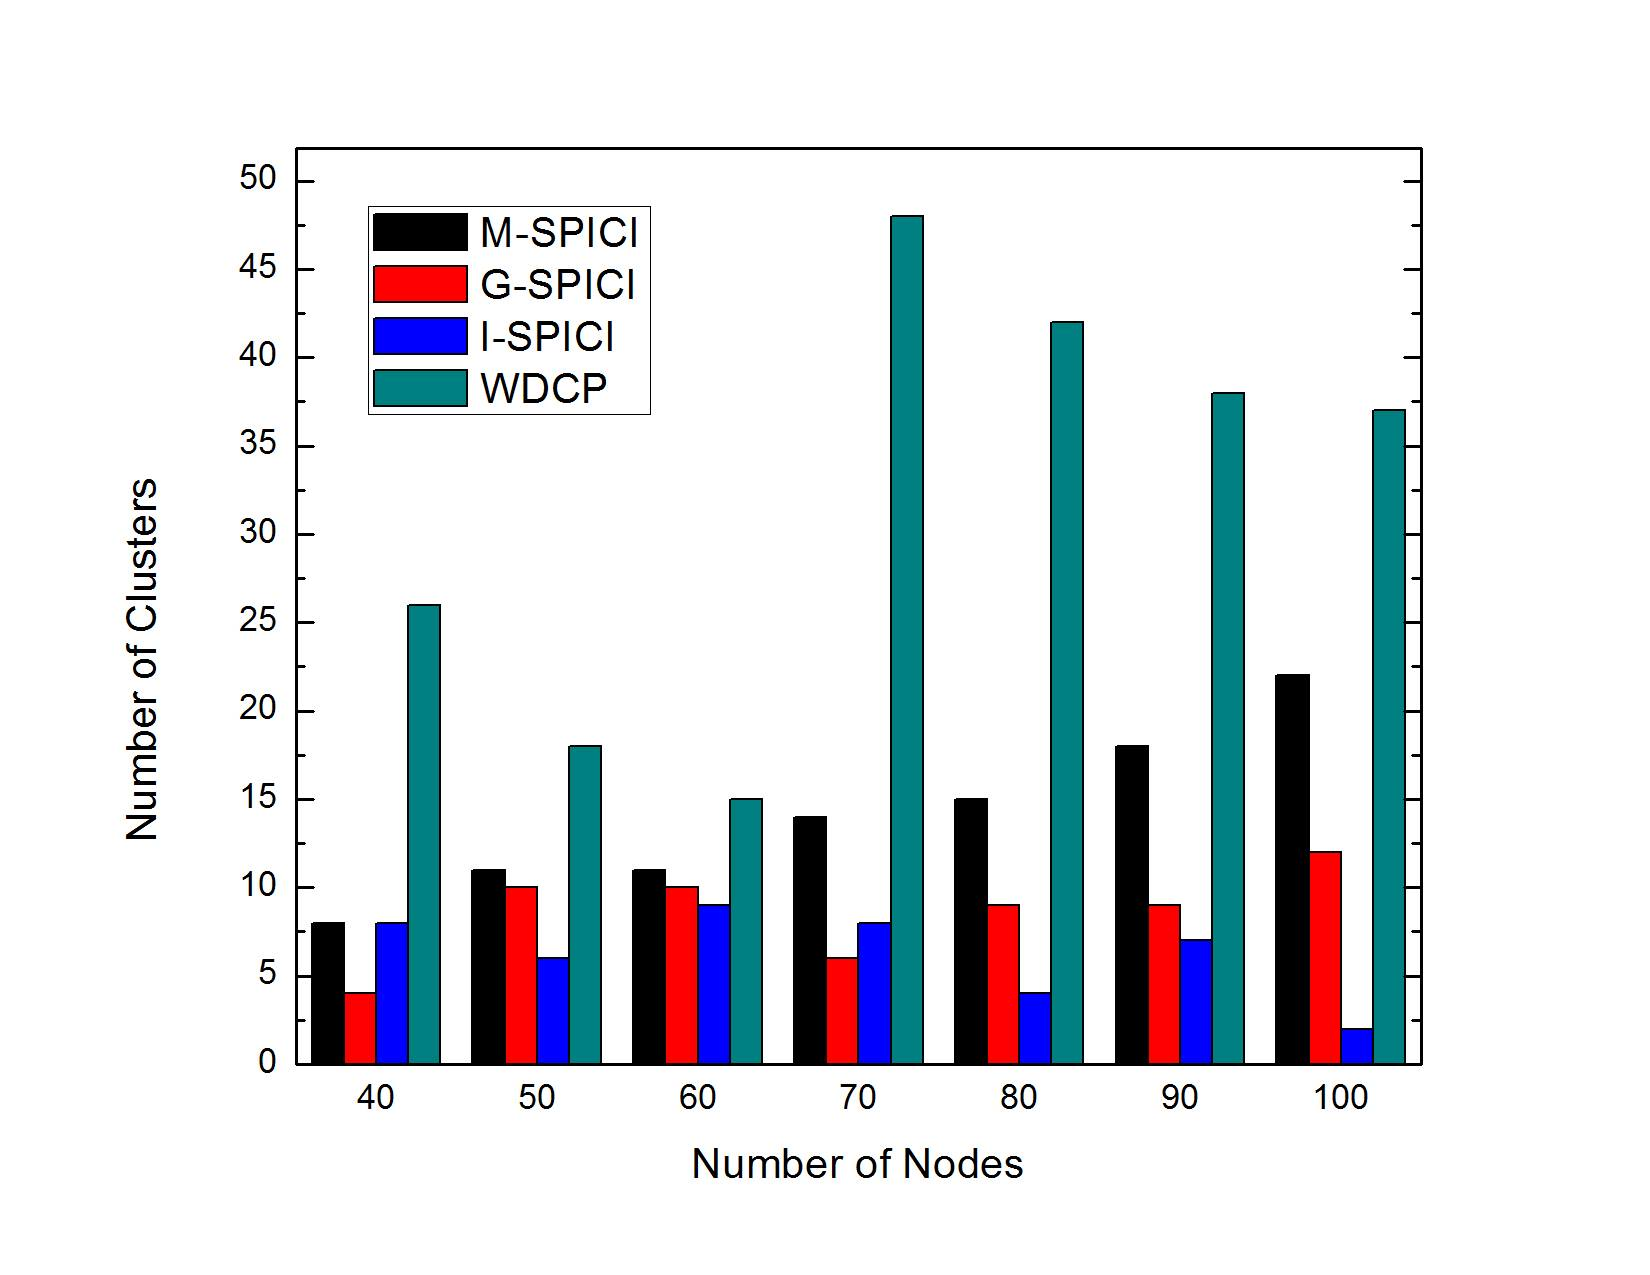
\includegraphics[width=\linewidth]{wbar.jpg}
	\caption{Comparison of the number of controllers $k$, for algorithms WDBCP, G-SPICi, I-SPICi and M-SPICi.}
	\label{fig:wbar}
\end{figure}


In figure \ref{fig:wgraph} we can see that WDBCP gives better results than our proposed algorithms in terms of $m_{latency}$, but from the figure \ref{fig:wbar} we can see that WDBCP gives a very high number of clusters than that of our proposed algorithms. This is acceptable when the cost of installing a controller is trivial, but in reality it is not feasible to accommodate the installment cost of so many controllers. Therefore, we compare our proposed algorithms with WDBCP in terms of $k*m_{latency}$ in figure \ref{fig:wgraphmul} for different scenarios to take into consideration the number of controllers $k$. If we consider the cost of each controller as constant $c$, then the cost of controller installment for a network is $k*c$. So the cost-latency product of a network is $c*k*m_{latency}$. As for each network the same constant is multiplied, we omitted $c$ and used $k*m_{latency}$ to represent the cost-latency product of a network.

We can see from \ref{fig:wgraphmul} that, I-SPICi and G-SPICi gives better result for all scenarios of table \ref{table:networks}, and our proposed algorithms outperform DBCP in terms of cost-latency product. For scenario 3 when number of nodes is 60, I-SPICi and G-SPICi give the same result. For scenarios 1 and 4, where nodes are 40 and 70 respectively, G-SPICi outperforms other algorithms. For other scenarios I-SPICi outperforms all other algorithms.

\begin{figure}
	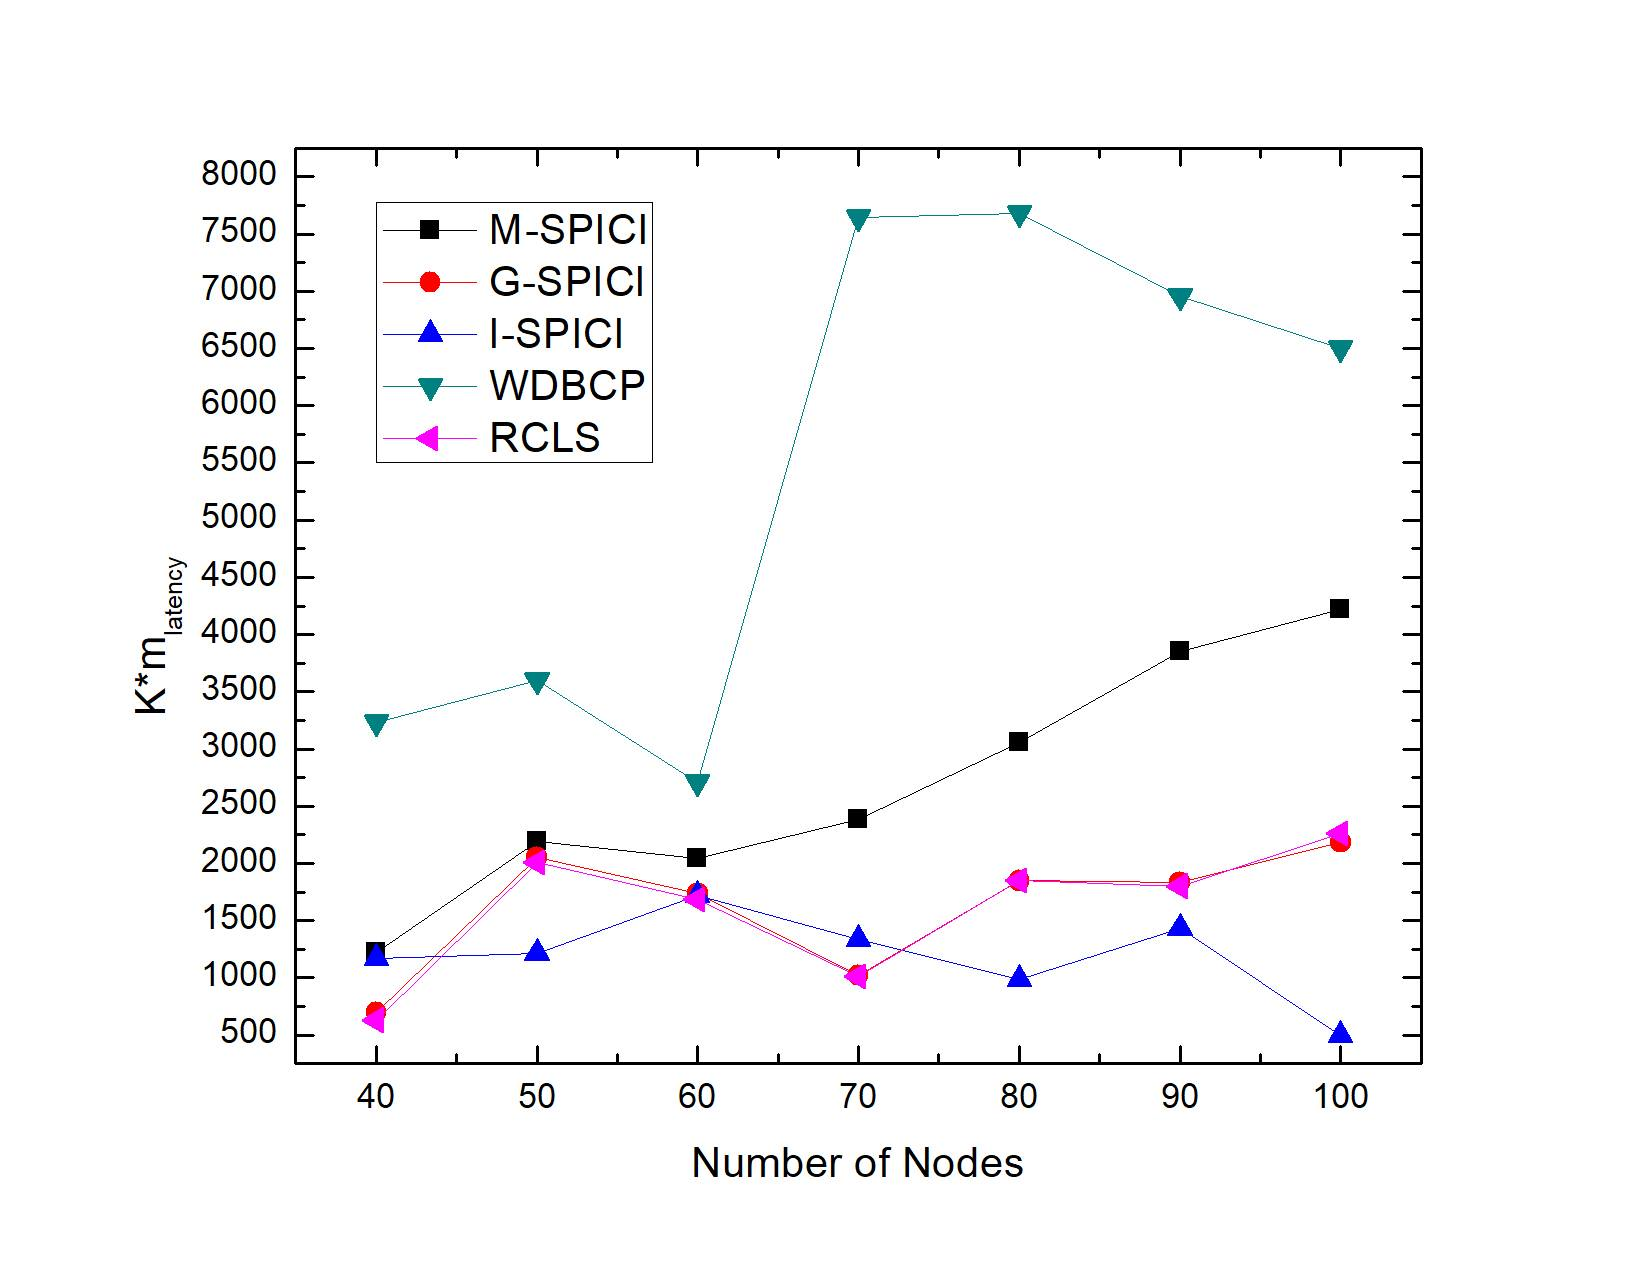
\includegraphics[width=\linewidth]{wgraphmul.jpg}
	\caption{Comparison of DBCP, G-SPICi, M-SPICi, I-SPICi and RCLS on weighted networks using $m^{latency}$ as performance metric.}
	\label{fig:wgraphmul}
\end{figure}

Our proposed algorithm RCLS is traffic-aware as it can re-cluster a network where the controllers are already selected. If we represent the edge values as incoming or outgoing traffic for a link between two switches, after the controllers are placed and the traffic of the network changes, RCLS can change the clusters when the graph edge values are updated according to changing traffic.

\subsection{Analysis of K}
The number of clusters or the value of $k$ is different for each algorithm. One of the questions which define the NP-Hard problem CPP is - \emph{How many controllers?}. The more we increase the value of $k$ the better is the result of the simulation. Therefore the best simulation result is obtained when $k=|S|$, where $|S|$ is the number of switches in the network. When all the switches are controllers, the latency of the network is minimum. However, this is not feasible as the cost of installing so many controllers is much more than required.

In figure \ref{fig:kanalysis} we have presented the results of RCLS on weighted graphs of different number of switches. For each network graph, the value of $k$ is increased from $1$ to $|S|$, where $S$ is the total number of switches in the network. As discussed, the value of $m_{latency}$ decreases with increasing $k$. We have to select a $k$ so that the latency of the network and the cost of installing the controllers is minimized. We have to select $k$ such that increasing the value of $k$ does negligible improvement compared to previous increases of $k$. We need to determine a threshold of improvement, although this might be different in different scenarios and depends on the need of the network operator. Therefore our proposed algorithm RCLS will cluster the network optimally based on the value of $k$ given by the network operator.

\begin{figure}
	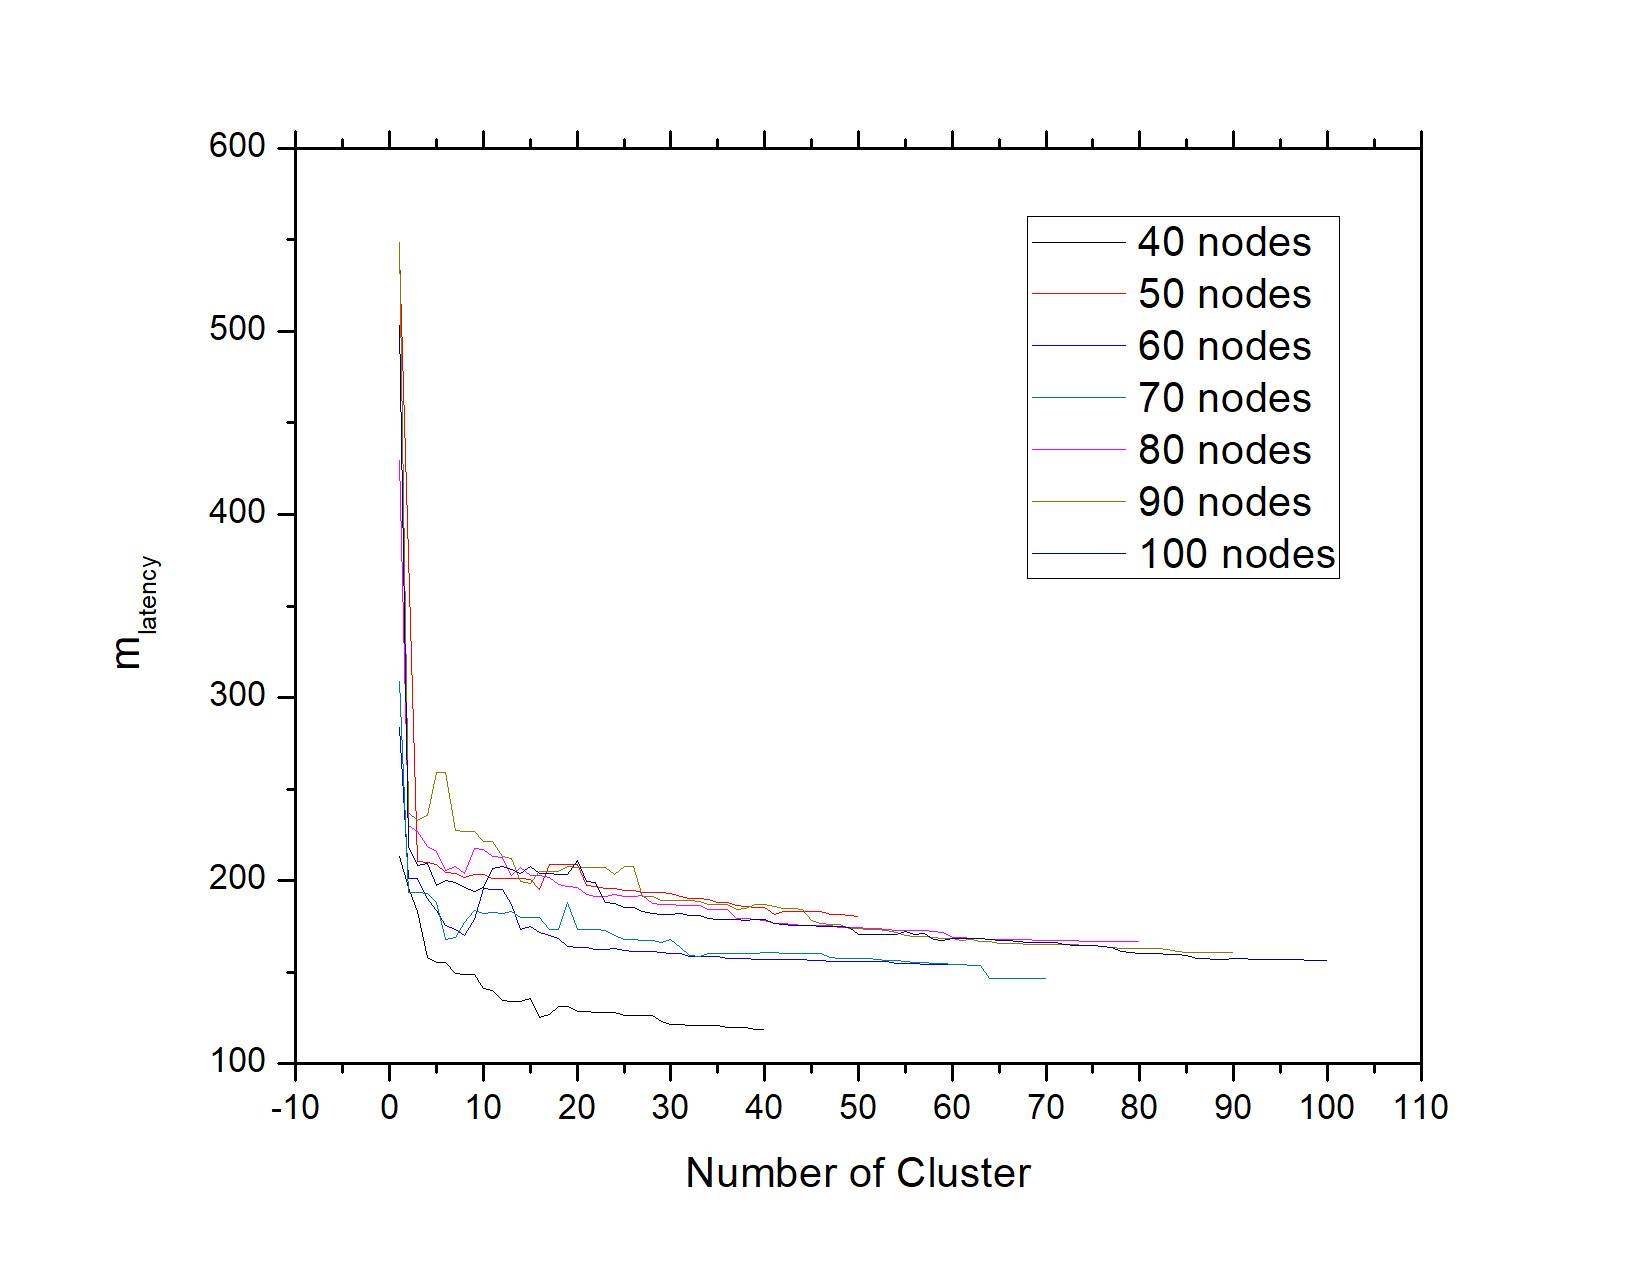
\includegraphics[width=\linewidth]{kanalysis.jpg}
	\caption{Comparison of DBCP, G-SPICi, M-SPICi, I-SPICi and RCLS on weighted networks using $m^{latency}$ as performance metric.}
	\label{fig:kanalysis}
\end{figure}


\section{Conclusion} \label {conclusion}
In this paper we address the Controller Placement Problem (CPP) of SDN. We have investigated one renowned algorithm DBCP \cite{dbcp2017} that addresses the same research problem. DBCP is for unweighted graph where it uses hop count as the distance metric. Our proposed algorithm RCLS outperforms DBCP in terms of latency for unweighted graph. However, un-weighted graph is not a good representation of a real network. Being inspired by another famous protein clustering algorithm SPICi \cite{spici2010} we propose 3 algorithms for weighted Graph. We have validated our result through extensive simulations. The simulation results suggest that our proposed algorithms outperform the weighted variant of the existing DBCP algorithm in terms of cost and latency. Our proposed algorithms also have polynomial time complexity.
\section*{References}

\bibliography{mybibfile}

\end{document}